%----------------------------------------------------------------------------------------
%	PACKAGES AND OTHER DOCUMENT CONFIGURATIONS
%----------------------------------------------------------------------------------------

\documentclass[a4paper]{article}

\usepackage[version=4]{mhchem}
\usepackage[T1]{fontenc} % Use 8-bit encoding that has 256 glyphs
\usepackage{lmodern}
\usepackage[hyphens]{url}
\usepackage{subcaption}
\usepackage{graphicx}
\linespread{1.05} % Line spacing - Palatino needs more space between lines
\usepackage{microtype} % Slightly tweak font spacing for aesthetics
\usepackage[spanish]{babel} % Language hyphenation and typographical rules
\usepackage[numbib,notlof,notlot,nottoc]{tocbibind} % Shows bibliography as a section
\usepackage[hmarginratio=1:1,top=32mm,columnsep=20pt]{geometry} % Document margins
\usepackage[section]{placeins}
\usepackage{float}
\usepackage{booktabs} % Horizontal rules in tables
\usepackage{enumitem} % Customized lists
\usepackage{fancyhdr} % Headers and footers
\usepackage{amssymb} 

\pagestyle{fancy} % All pages have headers and footers
\fancyhead{} % Blank out the default header
\fancyfoot{} % Blank out the default footer
\fancyhead[C]{Ejercicios resueltos del curso "GR" (Matthias Blau) $\bullet$ Ignacio Poggi} % Custom header text
\fancyfoot[C]{\thepage} % Custom footer text

\usepackage{titling} % Customizing the title section
\usepackage{hyperref} % For hyperlinks in the PDF

%----------------------------------------------------------------------------------------
%	TITLE SECTION
%----------------------------------------------------------------------------------------

\setlength{\droptitle}{-4\baselineskip} % Move the title up

\title{Ejercicios resueltos del curso "General Relativity", dado por Matthias Blau} % Article title
\author{%
\textsc{Ignacio Poggi} \\[1ex] % Your name
\normalsize \href{mailto:ignaciop.3@gmail.com}{ignaciop.3@gmail.com} % Your email address
}

\date{\today} % Leave empty to omit a date
\renewcommand{\maketitlehookd}{%
\begin{abstract}
\noindent Algunas ejercicios del curso, dictado en varios a\~nos, para comprender un poco mejor las bases de la Relatividad General. M\'as info: \href{http://www.blau.itp.unibe.ch/GREX/hs23.html}{http://www.blau.itp.unibe.ch/GREX/hs23.html}
\end{abstract}
}

%----------------------------------------------------------------------------------------

\begin{document}
\maketitle

% Print the title


%----------------------------------------------------------------------------------------
%	INCLUDES
%----------------------------------------------------------------------------------------
\section{TP1}
\subsection{M\'etricas, elementos de l\'inea y transformaciones de coordenadas}

Bajo una transformaci\'on de coordenadas a partir de coordenadas cartesianas (o inerciales) $\xi^{a} = \xi^{a}(x^{\mu})$, las m\'etricas euclidiana $\delta_{ab}$ o la de Minkowski $\eta_{ab}$ se transforman en una nueva
m\'etrica $g_{\mu \nu}$, de tal manera que las distancias propias son invariantes,

\begin{equation}
    (\delta_{ab}, \eta_{ab})d\xi^{a}d\xi^{b} = g_{\mu \nu}dx^{\mu}dx^{\nu} \iff g_{\mu \nu} = J_{\mu}^{a}J_{\nu}^{b}(\delta_{ab}, \eta_{ab})
    \label{eq1}
\end{equation}

con $J_{\mu}^{a} = \frac{\partial \xi^{a}}{\partial x^{\mu}}$, la matriz Jacobiana de la transformaci\'on.\\

\subsubsection{M\'etricas en 2D}

Considere el siguiente elemento de l\'inea bidimensional

\begin{equation}
    ds^{2} = (dy^{1})^{2} + (dy^{2})^{2} + 2ady^{1}dy^{2}
    \label{eq2}
\end{equation}

con $a \in \mathbb{R}$ constante.

\begin{itemize}
    \item Muestre que esta m\'etrica es no degenerada para $a \neq \pm 1$.
    \item Muestre que, para $a^{2} < 1$, la m\'etrica est\'a relacionada con la Euclideana $ds^{2} = (dx^{1})^{2} + (dx^{2})^{2}$ mediante la transformaci\'on.

    \begin{equation}
        x^{1} = \sqrt{1 - a^{2}}y^{1} \ , \ x^{2} = ay^{1} + y^{2}
        \label{eq3}
    \end{equation}

    \item Muestre que, para $a^{2} > 1$, la m\'etrica est\'a relacionada con la Lorentziana $ds^{2} = -dt^{2} + dx^{2}$ mediante alguna transformaci\'on.
\end{itemize}

\textbf{Soluci\'on:}\\

Es f\'acil ver que la m\'etrica adopta la siguiente forma matricial

$$g_{\mu \nu} =
    \begin{pmatrix}
    g_{y^{1}y^{1}} & g_{y^{1}y^{2}}\\
    g_{y^{2}y^{1}} & g_{y^{2}y^{2}}
    \end{pmatrix}
 = 
    \begin{pmatrix}
    1 & a\\
    a & 1
    \end{pmatrix}
$$\\

Luego, $g = \det(g_{\mu \nu}) = 1 - a^{2}$. Como $a \neq \pm 1$, entonces $g \neq 0$, por lo tanto la m\'etrica es no degenerada. $\checkmark$\\

Para $a^{2} > 1$, invertimos las transformaciones dadas (\ref{eq3}) en funci\'on de $y^{1}$ e $y^{2}$:

$$y^{1} = \frac{x^{1}}{\sqrt{1 - a^{2}}}$$

$$y^{2} = x^{2} - ay^{1} = x^{2} - a\frac{x^{1}}{\sqrt{1 - a^{2}}}$$

$$\Rightarrow dy^{1} = \frac{dx^{1}}{\sqrt{1 - a^{2}}} \ , \ dy^{2} = dx^{2} - a\frac{dx^{1}}{\sqrt{1 - a^{2}}}$$

Reemplazando esto en (\ref{eq2}), obtenemos

$$ds^{2} = \bigg(\frac{dx^{1}}{\sqrt{1 - a^{2}}}\bigg)^{2} + \bigg(dx^{2} - a\frac{dx^{1}}{\sqrt{1 - a^{2}}}\bigg)^{2} + 2a\bigg(\frac{dx^{1}}{\sqrt{1 - a^{2}}}\bigg)\bigg(dx^{2} - a\frac{dx^{1}}{\sqrt{1 - a^{2}}}\bigg)$$

$$ds^{2} = \frac{(dx^{1})^{2}}{1 - a^{2}} + (dx^{2})^{2} - 2a\frac{dx^{1}}{\sqrt{1 - a^{2}}}dx^{2} +  a^{2}\frac{(dx^{1})^{2}}{1 - a^{2}} + 2a\frac{dx^{1}}{\sqrt{1 - a^{2}}}dx^{2} - 2a^{2}\frac{(dx^{1})^{2}}{1 - a^{2}}$$

$$\Rightarrow ds^{2} = (1 - a^{2})\frac{(dx^{1})^{2}}{1 - a^{2}} + (dx^{2})^{2} = (dx^{1})^{2} + (dx^{2})^{2} \ \checkmark$$

Para $a^{2} < 1$, se proponen las siguientes transformaciones:

$$t = \sqrt{a^{2} - 1}y^{1} \Rightarrow dt = \sqrt{a^{2} - 1}dy^{1}$$

$$x = ay^{1} + y^{2} \Rightarrow dx = ady^{1} + dy^{2}$$

Haciendo el mismo c\'alculo que en el punto anterior, obtenemos

$$ds^{2} = -dt^{2} + dx^{2}$$

\subsubsection{M\'etrica de Rindler}

Considere la m\'etrica de Minkowski (1+1)-dimensional con elemento de l\'inea $ds^{2} = -dt^{2} + dx^{2}$, y las \textit{coordenadas de Rindler} $(T, X)$ definidas como

\begin{equation}
    t = X\sinh{T} \ , \ x = X\cosh{T}
    \label{eq4}
\end{equation}

con $a \in \mathbb{R}$ constante.

\begin{itemize}
    \item Determine la m\'etrica o elemento de l\'inea en estas coordenadas.
    \item Muestre que las l\'ineas $T = cte$, $X = cte$ son l\'ineas rectas que pasan por el origen o hiperbolas (en un diagrama $(t, x)$), respectivamente.
\end{itemize}

\textbf{Soluci\'on:}\\

Diferenciando las nuevas coordenadas

$$dt = dX\sinh{T} + X\cosh{T}dT$$

$$dx = dX\cosh{T} + X\sinh{T}dT$$\\

Elevando al cuadrado ambas igualdades

$$dt^{2} = (dX\sinh{T} + X\cosh{T}dT)^{2} = dX^{2}\sinh^{2}{T} + 2XdX\sinh{T}\cosh{T}dT + X^{2}\cosh^{2}{T}dT^{2}$$

$$dx^{2} = (dX\cosh{T} + X\sinh{T}dT)^{2} = dX^{2}\cosh^{2}{T} + 2XdX\cosh{T}\sinh{T}dT + X^{2}\sinh^{2}{T}dT^{2}$$\\

Reemplaz\'andolas en $ds^{2} = -dt^{2} + dx^{2}$:

$$ds^{2} = -dX^{2}\sinh^{2}{T} - 2XdX\sinh{T}\cosh{T}dT - X^{2}\cosh^{2}{T}dT^{2}$$
$$+ dX^{2}\cosh^{2}{T} + 2XdX\cosh{T}\sinh{T}dT + X^{2}\sinh^{2}{T}dT^{2}$$\\
$$\Rightarrow ds^{2} = (dX^{2} - X^{2}dT^{2})(\cosh^{2}{T} - \sinh^{2}{T}) =  - X^{2}dT^{2} + dX^{2} \ \checkmark$$\\

Para $T = T_{0}$ constante, las ecuaciones (\ref{eq4}) nos quedan:

$$t = X\sinh{T_{0}} \ , \ x = X\cosh{T_{0}}$$

$$\Rightarrow t = \frac{x}{\cosh{T_{0}}}\sinh{T_{0}} = x\tanh{T_{0}}\  \checkmark$$

es la ecuaci\'on de una recta que pasa por el origen.\\

Tomando $X = X_{0}$ constante, obtenemos de las ecuaciones (\ref{eq4}):

$$t = X_{0}\sinh{T} \ , \ x = X_{0}\cosh{T}$$

$$\Rightarrow t^{2} = X_{0}^{2}\sinh^{2}{T} \ , \ x^{2} = X_{0}^{2}\cosh^{2}{T}$$

Restando ambos cuadrados

$$t^{2} - x^{2} = X_{0}^{2}(\sinh^{2}{T} - \cosh^{2}{T}) = X_{0}^{2}\ \checkmark$$

describiendo una hip\'erbola en el plano $(t, x)$.

\begin{figure}[H]
    \centering
    \begin{subfigure}[b]{0.5\linewidth}
        \fbox{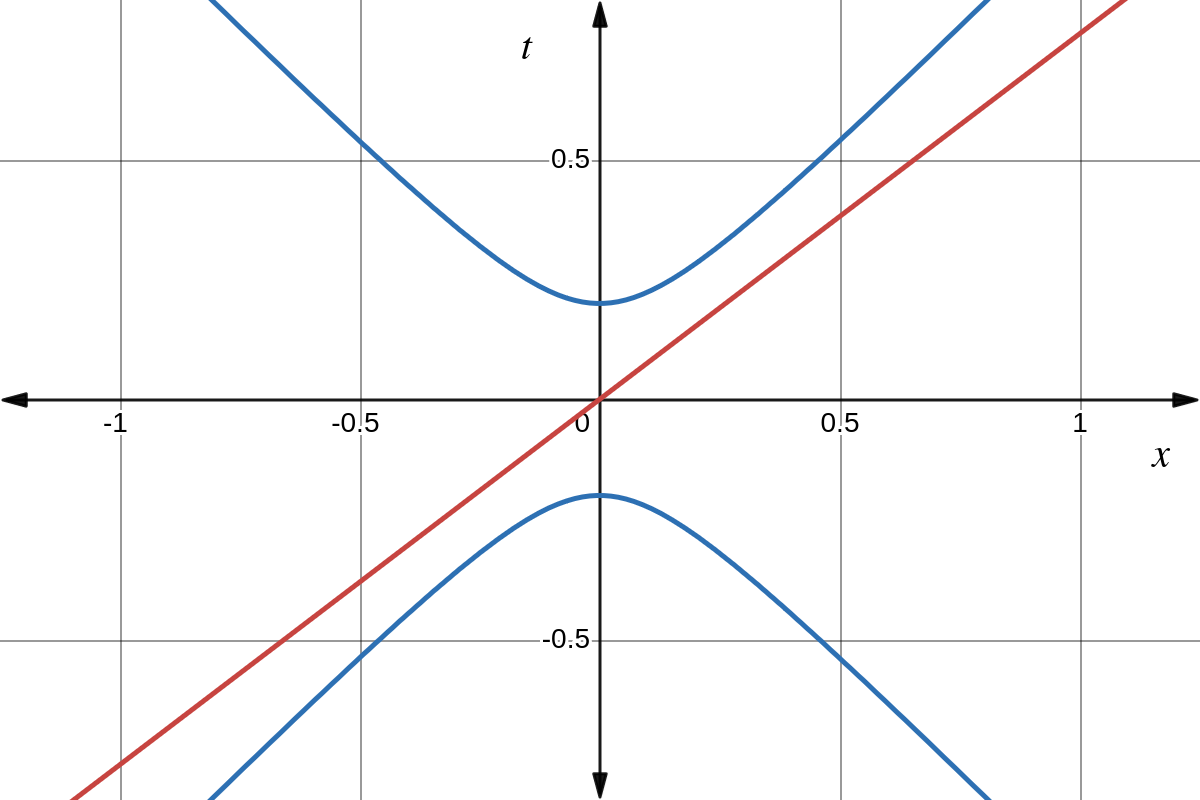
\includegraphics[width=\linewidth]{A1/a1_ex1.png}}
    \end{subfigure}
    \caption{Recta $t = x\tanh{T_{0}}$ (rojo) e hip\'erbola $t^{2} - x^{2} = X_{0}^{2}$ (azul), con constantes $T_{0} = 1$ y $X_{0} = 0.2$, respectivamente.}
    \label{fig:cap1_trappedsurface}
\end{figure}

\subsection{Geod\'esicas I}

\subsubsection{Geod\'esicas y ecuaciones de Euler-Lagrange}

Muestre que las ecuaciones de Euler-Lagrange

\begin{equation}
    \frac{d}{d\lambda}\frac{\partial \mathcal{L}}{\partial x'^{\mu}} - \frac{\partial \mathcal{L}}{\partial x^{\mu}} = 0
    \label{eq5}
\end{equation}

para el Lagrangiano

\begin{equation}
    \mathcal{L} = \frac{1}{2}g_{\mu \nu}\frac{dx^{\mu}}{d\lambda}\frac{dx^{\nu}}{d\lambda} = \frac{1}{2}g_{\mu \nu}x'^{\mu}x'^{\nu}
    \label{eq6}
\end{equation}

son las ecuaciones geod\'esicas

\begin{equation}
    \frac{d^{2}x^{\mu}}{d\lambda^{2}} + \Gamma^{\mu}_{\nu \lambda}\frac{dx^{\nu}}{d\lambda}\frac{dx^{\lambda}}{d\lambda} = 0
    \label{eq7}
\end{equation}

donde los \textit{s\'imbolos de Christoffel} $\Gamma^{\mu}_{\nu \lambda}$ asociados a la m\'etrica $g_{\mu \nu}$ se definen como

\begin{equation}
    \Gamma^{\mu}_{\nu \lambda} = g^{\mu \rho}\Gamma_{\rho \nu \lambda} = \frac{1}{2}g^{\mu \rho}(\partial_{\lambda}g_{\nu \rho} + \partial_{\nu}g_{\rho \lambda} - \partial_{\rho}g_{\nu \lambda})
    \label{eq8}
\end{equation}\\

\textbf{Soluci\'on:}\\

Calculemos el primer t\'ermino de la ecuaci\'on (\ref{eq5}) usando (\ref{eq6}):

$$\frac{d}{d\tau}\bigg(\frac{\partial \mathcal{L}}{\partial x'^{\gamma}}\bigg) = \frac{d}{d\tau}\bigg(g_{\gamma \nu}x'^{\nu}\bigg)$$

El segundo t\'ermino queda de la siguiente manera:

$$\frac{\partial \mathcal{L}}{\partial x^{\gamma}} = \frac{1}{2}\partial_{\gamma}g_{\mu \nu}x'^{\mu}x'^{\nu}$$\\

Juntando todo en (\ref{eq5})

$$\frac{d}{d\tau}(g_{\gamma \nu}x'^{\nu}) - \frac{1}{2}\partial_{\gamma}g_{\mu \nu}x'^{\mu}x'^{\nu} = \frac{d}{d\tau}(g_{\gamma \nu})x'^{\nu} + g_{\gamma \nu}\frac{d}{d\tau}(x'^{\nu}) - \frac{1}{2}\partial_{\gamma}g_{\mu \nu}x'^{\mu}x'^{\nu}$$\\

Veamos por separado los dos primeros t\'erminos del lado derecho de esta \'ultima igualdad:

$$\frac{d}{d\tau}(g_{\gamma \nu})x'^{\nu} = \partial_{\mu}g_{\gamma \nu}x'^{\mu}x'^{\nu}$$

$$g_{\gamma \nu}\frac{d}{d\tau}(x'^{\nu}) = g_{\gamma \nu}x''^{\nu}$$\\

Luego

$$\partial_{\mu}g_{\gamma \nu}x'^{\mu}x'^{\nu} + g_{\gamma \nu}x''^{\nu} - \frac{1}{2}\partial_{\gamma}g_{\mu \nu}x'^{\mu}x'^{\nu} = 0$$

$$\Rightarrow  \frac{1}{2}(\partial_{\mu} g_{\gamma \nu} + \partial_{\nu} g_{\gamma \beta})x'^{\mu}x'^{\nu} + g_{\gamma \nu}x''^{\nu} - \frac{1}{2}\partial_{\gamma}g_{\mu \nu}x'^{\mu}x'^{\nu} = 0$$\\

(el primer t\'ermino se puede escribir as\'i porque $x'^{\mu}x'^{\nu} = x'^{\nu}x'^{\mu}$ es sim\'etrico). Reagrupando el primero y \'ultimo del lado izquierdo:

$$g_{\gamma \nu}x''^{\nu} + \frac{1}{2}(\partial_{\mu} g_{\gamma \nu} + \partial_{\nu} g_{\gamma \beta} - \partial_{\gamma}g_{\mu \nu})x'^{\mu}x'^{\nu} = 0$$\\

El segundo t\'ermino es el \textit{s\'imbolo de Christoffel de primer tipo} $\Gamma_{\gamma \mu \nu}$, por lo tanto

$$g_{\gamma \nu}x''^{\nu} + \Gamma_{\gamma \mu \nu}x'^{\mu}x'^{\nu} = 0$$\\

Si multiplicamos por $g^{\gamma \rho}$ (m\'etrica inversa) para elevar uno de los \'indices, obtenemos finalmente (\ref{eq7}):

$$g^{\gamma \rho}g_{\rho \nu}x''^{\nu} + g^{\gamma \rho}\Gamma_{\rho \mu \nu}x'^{\mu}x'^{\nu} = 0$$\\

$$\Rightarrow x''^{\gamma} + \Gamma^{\gamma}_{\mu \nu}x'^{\mu}x'^{\nu} = 0 \ \checkmark$$\\

\subsubsection{$\mathcal{L}$ es una constante de movimiento}

Muestre que $\mathcal{L}$ es constante a lo largo de cualquier geod\'esica, es decir

\begin{equation}
    \frac{d}{d\lambda}\bigg( g^{\mu \nu}\frac{dx^{\mu}}{d\lambda}\frac{dx^{\nu}}{d\lambda} \bigg) = 0
    \label{eq9}
\end{equation}

para $x^{\mu}(\lambda)$ soluci\'on de la ecuaci\'on geod\'esica.

¿Cual es la simetr\'ia, por el teorema de Noether, que da lugar a esta constante de movimiento?\\

\textbf{Soluci\'on:}\\

Es bastante autom\'atico si procedemos como en el punto anterior. Nuevamente

$$\frac{d}{d\tau}(g_{\mu \nu}) = \partial_{\gamma}g_{\mu \nu}x'^{\gamma}$$

$$\Rightarrow \frac{d\mathcal{L}}{d\tau} = \partial_{\gamma}g_{\mu \nu}x'^{\mu}x'^{\nu}x'^{\gamma} + 2g_{\mu \nu}x''^{\mu}x'^{\nu}$$\\

Usando la identidad $\partial_{\gamma}g_{\mu \nu} = \Gamma_{\mu \nu \gamma} + \Gamma_{\nu \mu \gamma}$, entonces $\partial_{\gamma}g_{\mu\nu}x'^{\mu}x'^{\nu}x'^{\gamma} = 2\Gamma_{\nu \mu \gamma}x'^{\mu}x'^{\nu}x'^{\gamma}$. Por lo tanto

$$\frac{d\mathcal{L}}{d\tau} = 2(g_{\nu \mu}x''^{\mu} + \Gamma_{\nu \mu \gamma}x'^{\mu}x'^{\gamma})x'^{\nu}$$

la cual se anula por ser una soluci\'on de la geod\'esica.\\

La simetr\'ia que corresponde a esta cantidad conservada es la traslaci\'on en $\tau$ (dado que el Lagrangiano no depende expl\'icitamente de este par\'ametro, la energ\'ia correspondiente se conserva).
\newpage
\section{TP2}
\subsection{S\'imbolos de Christoffel y transformaciones de coordenadas}

\begin{itemize}
    \item Utilice el comporamiento tensorial de la siguiente m\'etrica bajo la transformaci\'on de coordenadas $x^{\mu} \rightarrow y^{\alpha}(x^{\mu})$,

        \begin{equation}
            g_{\alpha \beta} = J^{\mu}_{\alpha}J^{\nu}_{\beta}g_{\mu \nu}
            \label{eq10}
        \end{equation}

        para mostrar que los s\'imbolos de Christoffel transforman como 

        \begin{equation}
            \Gamma^{\alpha}_{\beta \gamma} = J^{\alpha}_{\mu}J^{\nu}_{\beta}J^{\lambda}_{\gamma}\Gamma^{\mu}_{\nu \lambda} + J^{\alpha}_{\mu}J^{\mu}_{\beta \gamma}
            \label{eq11}
        \end{equation}

    \item Muestre que, como consecuencia de (\ref{eq11}), $\Ddot{x}^{\mu} +  \Gamma^{\mu}_{\nu \lambda}\Dot{x}^{\nu}\Dot{x}^{\delta}$ transforma como un \textit{vector} bajo transformaciones de coordenadas, es decir

    $$\Ddot{y}^{\mu} +  \Gamma^{\mu}_{\nu \lambda}\Dot{y}^{\nu}\Dot{y}^{\delta} = J^{\alpha}_{\mu}(\Ddot{x}^{\mu} +  \Gamma^{\mu}_{\nu \lambda}\Dot{x}^{\nu}\Dot{x}^{\delta})$$

    Ayuda: puede usar la siguiente identidad

    $$J^{\alpha}_{\mu}J^{\mu}_{\beta} = \delta_{\alpha}^{\beta}$$
\end{itemize}

\textbf{Soluci\'on:}\\

Por definici\'on, el s\'imbolo de Christoffel de primer tipo se escribe en funci\'on de las derivadas de la m\'etrica de la siguiente manera

$$2\Gamma_{\alpha \beta \gamma} = \partial_{\gamma}g_{\alpha \beta} + \partial_{\beta}g_{\alpha \gamma} - \partial_{\alpha}g_{\beta \gamma}$$\\

Escribamos la tranformaci\'on del primer t\'ermino de acuerdo a (\ref{eq10}), y los dos restantes seguir\'an la misma l\'inea (con los \'indices correspondientes)

$$ \partial_{\gamma}g_{\alpha \beta} =  \partial_{\gamma}(J^{\mu}_{\alpha}J^{\nu}_{\beta}g_{\mu \nu}) = \partial_{\lambda}g_{\mu \nu}J^{\mu}_{\alpha}J^{\nu}_{\beta}J^{\lambda}_{\gamma} + (J^{\mu}_{\alpha \gamma}J^{\nu}_{\beta} + J^{\nu}_{\beta}J^{\nu}_{\beta \gamma})g_{\mu \nu}$$\\

Aqu\'i se utilizo la regla de la cadena de la derivada (primero en la m\'etrica, teniendo en cuenta las transformaci\'oon $\partial_{\gamma} = J^{\lambda}_{\gamma}\partial_{\lambda}$; y luego en las $J$ con $J^{\mu}_{\beta \gamma} = \partial_{\beta}J^{\mu}_{\gamma} = \frac{\partial^{2}x^{\mu}}{\partial y^{\beta}y^{\gamma}}$). Por lo tanto:

$$2\Gamma_{\alpha \beta \gamma} = \partial_{\gamma}g_{\alpha \beta} + \partial_{\beta}g_{\alpha \gamma} - \partial_{\alpha}g_{\beta \gamma} = 2J^{\mu}_{\alpha}J^{\nu}_{\beta}J^{\lambda}_{\gamma}\Gamma_{\mu \nu \lambda} + (J^{\mu}_{\alpha \gamma}J^{\nu}_{\beta} + J^{\nu}_{\beta}J^{\nu}_{\beta \gamma} + J^{\mu}_{\alpha \beta}J^{\nu}_{\gamma} + J^{\mu}_{\alpha}J^{\nu}_{\gamma \beta} - J^{\mu}_{\beta \alpha}J^{\nu}_{\gamma} - J^{\mu}_{\beta}J^{\nu}_{\gamma \alpha})g_{\mu \nu}$$\\

En esta igualdad, los siguientes t\'erminos se cancelan entre s\'i: el tercero y quinto dado que $J^{\mu}_{\alpha \beta}$ es sim\'etrica; el primero y sexto porque $J^{\mu}_{\alpha \gamma}$ y $g_{\mu \nu}$ son sim\'etricas. El segundo y cuarto se suman, dando lugar a

$$\Gamma_{\alpha \beta \gamma} = J^{\mu}_{\alpha}J^{\nu}_{\beta}J^{\lambda}_{\gamma}\Gamma_{\mu \nu \lambda} + J^{\mu}_{\alpha}J^{\nu}_{\beta \gamma}g_{\mu \nu}$$

Si multiplicamos esta \'ultima igualdad por la m\'etrica inversa $g^{\alpha \delta} = g^{\sigma \rho}J^{\alpha}_{\sigma}J^{\delta}_{\rho}$, obtenemos el resultado buscado:

$$\Gamma^{\alpha}_{\beta \gamma} = g^{\alpha \delta}\Gamma_{\delta \beta \gamma} = J^{\mu}_{\alpha}J^{\nu}_{\beta}J^{\lambda}_{\gamma}\Gamma^{\mu}_{\nu \lambda} + J^{\mu}_{\alpha}J^{\nu}_{\beta \gamma}g_{\mu \nu}\ \checkmark$$\\

Un ejemplo del uso de la ayuda del enunciado es en el c\'alculo del segundo t\'ermino al elevar el \'indice $\alpha$:

$$g^{\alpha \delta}J^{\mu}_{\delta}J^{\nu}_{\beta \gamma}g_{\mu \nu} = (g^{\sigma \rho}J^{\alpha}_{\sigma}J^{\delta}_{\rho})J^{\mu}_{\delta}J^{\nu}_{\beta \gamma}g_{\mu \nu} = g^{\sigma \rho}J^{\alpha}_{\sigma}(\delta^{\mu}_{\rho})J^{\nu}_{\beta \gamma}g_{\mu \nu} = g^{\sigma \mu}J^{\alpha}_{\sigma}J^{\nu}_{\beta \gamma}g_{\mu \nu} = \delta^{\sigma}_{\nu}J^{\alpha}_{\sigma}J^{\nu}_{\beta \gamma} = J^{\alpha}_{\nu}J^{\nu}_{\beta \gamma}$$\\

Las cuadrivelocidades tranforman como vectores, es decir

$$\Dot{y}^{\alpha} = J^{\alpha}_{\mu}\Dot{x}^{\mu}$$

Diferenciando nuevamente, y aplicando la regla de la cadena:

$$\Rightarrow \Ddot{y}^{\alpha} = J^{\alpha}_{\mu}\Ddot{x}^{\mu} + J^{\alpha}_{\mu \nu}\Dot{x}^{\mu}\Dot{x}^{\nu}$$

Reemplaz\'andolo en la geod\'esica, nos queda as\'i

$$\Ddot{y}^{\alpha} + \Gamma^{\alpha}_{\beta \gamma}\Dot{y}^{\beta}\Dot{y}^{\gamma} = J^{\alpha}_{\mu}(\Ddot{x}^{\mu} + \Gamma^{\mu}_{\nu \lambda}J^{\nu}_{\beta}J^{\lambda}_{\gamma}\Dot{y}^{\beta}\Dot{y}^{\gamma}) + J^{\alpha}_{\mu}J^{\mu}_{\beta \gamma}\Dot{y}^{\beta}\Dot{y}^{\gamma} + J^{\alpha}_{\mu \nu}\Dot{x}^{\mu}\Dot{x}^{\nu}$$

$$\Rightarrow \Ddot{y}^{\alpha} + \Gamma^{\alpha}_{\beta \gamma}\Dot{y}^{\beta}\Dot{y}^{\gamma} = J^{\alpha}_{\mu}(\Ddot{x}^{\mu} + \Gamma^{\mu}_{\nu \lambda}\Dot{x}^{\mu}\Dot{x}^{\nu}) + (J^{\alpha}_{\mu}J^{\mu}_{\beta \gamma} + J^{\alpha}_{\mu \nu}J^{\mu}_{\beta}J^{\nu}_{\gamma})\Dot{y}^{\beta}\Dot{y}^{\gamma}$$\\

El primer t\'ermino es el resultado buscado; el segundo es 0, ya que

$$0 = \partial_{\gamma}\delta^{\alpha}_{\beta} = \partial_{\gamma}(J^{\alpha}_{\mu}J^{\mu}_{\beta}) = J^{\alpha}_{\mu \nu}J^{\nu}_{\gamma}J^{\mu}_{\beta} + J^{\alpha}_{\mu}J^{\mu}_{\beta \gamma}$$

$$\Rightarrow \Ddot{y}^{\alpha} + \Gamma^{\alpha}_{\beta \gamma}\Dot{y}^{\beta}\Dot{y}^{\gamma} = J^{\alpha}_{\mu}(\Ddot{x}^{\mu} + \Gamma^{\mu}_{\nu \lambda}\Dot{x}^{\mu}\Dot{x}^{\nu})\ \checkmark$$
\newpage
\section{TP3}
\subsection{\'Algebra tensorial}

\subsection{El potencial geod\'esico efectivo}



%----------------------------------------------------------------------------------------


%----------------------------------------------------------------------------------------
%	REFERENCE LIST
%----------------------------------------------------------------------------------------
%\newpage
%\begin{thebibliography}{99} % Bibliography - this is intentionally simple in this template
 
%\end{thebibliography}


%----------------------------------------------------------------------------------------

\end{document}